
\documentclass[a4paper, 12pt]{article}
\usepackage{bm, array, graphicx, hyperref, amsmath, setspace, geometry, wrapfig}
\usepackage[font={footnotesize}]{caption}

\geometry{
a4paper,
total={170mm, 257mm},
left = 20mm,
top = 20mm
}

\begin{document}

\title{Cross relaxation mechanisms in fluorine-containing sample under conditions of DNP.}
\author{Dr Alexey Potapov\\
School of Physics and Astronomy\\
Sir Peter Mansfield Imaging Centre \\
\texttt{ alexey.potapov@nottingham.ac.uk}\\
tel: 0115 951 4739 }
\maketitle
 
\doublespacing
 
\section{Cross-relaxation in \textsuperscript{1}H- \textsuperscript{19}F system.}
While searching for optimal conditions of DNP in fluorinated samples, we stumbled upon a peculiar phenomenon, where after shutting down the MW irradiation, the \textsuperscript{19}F magnetization builds up rapidly to a value higher than thermal equilibrium, and then slowly approaches it. These observations suggest that \textsuperscript{19}F nuclei are in contact with some other reservoir of energy, which is colder than lattice. The most obvious candidate for such a reservoir are abundant protons. In an experiment where protons were saturated prior the measurement, the 19F magnetization does not overshoot to non-equilibrium values. In the following we'll try to take a closer look at the mechanisms, which might be responsible for this transfer process.
\section{NOE.}
The transfer process is somewhat similar to NOE (nuclear Overhauser effect), which was observed in solids quite a while ago. The latest reports published by the groups of Corzillius and Buntkowsky, describe NOE-like transfer of magnetization between protons and carbons under conditions of MAS DNP (magnetic field of 9.4 T and temperature 100 K). Such transfer is attributed to a motion of methyl groups, which is present even under such low temperatures. Similarly other reports of NOE in solids from the early days of NMR (Pines \& Waugh etc.) also attribute the transfer to some molecular motions. Our experiments however were carried at much lower temperatures of 1.4 K, where motions are quite suppressed. 
Our main hypothesis is that a tranfer between \textsuperscript{1}H and \textsuperscript{19}F  is caused by the presence of paramagnetic TEMPO radical. When we inadvertently replaced it with TEMPOL, we discovered that the \textsuperscript{1}H to \textsuperscript{19}F transfer was either significantly suppressed, or disappeared entirely. In order to show that in more detail we need to demonstrate what happens to the cross-relaxation effect, when TEMPO concentration varies.

******************

\textbf{In the following} we will start with the expression for the nuclear relaxation rate induced by electron flips, and we'll use it as a benchmark for comparing with other cross-relaxation rates. Then we will explore the second order corrections to the Hamiltonian due to a hyperfine interaction and demonstrate that they \textbf{could not} produce time-dependent terms leading to relaxation. Next, we will explore the flip-flop rates in a system of one electron, one hyperfine coupled nucleus and another dipolar coupled nucleus. We will show that the flip-flop rates are smaller than nuclear flip rate $\dfrac{1}{T_1}$, and thus could not produce significant effect over the lifetime of nuclear magnetization.

Finally, we will explore a model where nuclear flip-flops occur due to fast nuclear energy level crossings, produced by random electron spin jumps, and demonstrate that under certain conditions it might yield rather fast cross-relaxation rates.

******************

\section{Nuclear relaxation.}
In the following we estimate the rates of cross-relaxation based on the time-dependent perturbation theory (Ch. VIII.II.C in Abragam's book). Consider a two-level system, with $\vert i \rangle$ - initial, and $\vert f \rangle$ - final states, and the time-dependent perturbation to a system Hamiltonian $V(t) = \hat{A} f(t)$, where $\overline{f(t)} = 0$. The transfer rate from the $\vert i \rangle$ - to  $\vert f \rangle$ state can be calculated as:
\begin{equation} \label{eq:rate}
 W_{if} = \dfrac{ \vert A_{if} \vert ^2  }{\hbar^2} J(\omega_{if}) 
\end{equation}
where $\vert A_{if} \vert$ is the matrix element between the two states, and $J({\omega_{if}})$ is the spectral density at the transition frequency $\omega_{if} = \dfrac{E_f - E_i}{\hbar}$. For a stationary random process with exponentially decaying correlation function, the spectral density has the following form:
\begin{equation}
J(\omega) = \dfrac{\tau_c}{1+\omega^2\tau_c^2}, 
\end{equation} 
where $\tau_c$ is the correlation time of the random process.

The spin Hamiltonian of a nucleus coupled to an electron via a hyperfine interaction represented by a tensor $A_{i,j}$ can be written as:

\begin{equation}
       \mathcal{H} =  \omega_S \hat{S}_z + \sum \limits_{i,j=x,y,z} A_{ij} \hat{S}_i \hat{I}_j  - \omega_n \hat{I}_z \approx 
\end{equation}

Since the electron Zeeman interaction is stronger than any other interaction, the Hamiltonian can be projected along the $\hat{S}_z$ operator giving rise to the following expression:

\begin{equation}
\mathcal{H} =  \omega_S \hat{S}_z + A \hat{S}_z \hat{I}_z + B \hat{S}_z \hat{I}_x - \omega_n \hat{I}_z,
\end{equation}

where $A$ and $B$ are the secular and non-secular parts of the hyperfine interaction respectively. Electron spin $S = \dfrac{1}{2}$ undergoes rapid jumps with the correlation time $\tau_c$. According to Eq.\ref{eq:rate} the non-secular part of the hyperfine interaction would produce the nuclear relaxation rate (Ch. IX.II.A Abragam):

\begin{equation}\label{eq:nuclear__relax}
W_{n} =    \vert B \vert ^2 \dfrac{\tau_c}{1+\omega_n^2\tau_c^2},  \\
\end{equation}
  
Carr-Purcell-Meiboom-Gill experiments measuring nuclear $T_2$ were used earlier to determine electron correlation time $\tau_c$. In 40 mM solution of TEMPO radicals at 9.4 T magnetic field it was found to be $\tau_c approx$100 $\mu$s and be driven primarily by electron spin diffusion (Potapov et al. JMR 2012). At the 3.4 T magnetic field used in our experiments, the spectrum would become narrower by a factor of 3, thus effectively increasing the number of electron pairs undergoing spin diffusion flip-flops. On the other hand, our measurements are carried out at a lower temperature of 1.4 K, where electrons are strongly polarized ($\approx$ 91 \%polarization) thus reducing a number of flip-floping pairs by a factor of $\approx$5 compared to higher temperatures (Takahashi et al. PRL 2008, 101, 047601). Overall the effects of the magnetic field and temperature work in the opposite directions, thus leaving the correlation time at  about the same value of  $\tau_c \approx 100 \mu$s. 

 Given this correlation time, for most nuclei under our experimental conditions $\omega_n \tau_c \gg 1$, allowing the Eq.\ref*{eq:nuclear__relax} to be transformed as:
\begin{equation}
W_{n} \approx    \Big( \dfrac{B}{\omega_n} \Big) ^2 \dfrac{1}{\tau_c}  \\
\end{equation}

 In an actual sample containing many nuclei the spin diffusion averages the nuclear relaxation times of nuclei, except nuclei in the vicinity of electron which are detuned from the bulk by strong hyperfine interactions.



\section{Electron-mediated coupling between nuclei.}
In this section we will explore the effective internuclear coupling emerging due to interaction of nuclei with the same electron.
We will include the hyperfine interactions for both nuclei, while neglecting the dipolar interaction between them as shown schematically in Figure \ref{fig:coupling}B. In effect, this describes a situation where nuclei are spatially remote from one another. The Hamiltonian for such a system would therefore be in the following form:
\begin{equation}
\mathcal{H} =  \omega_S \hat{S}_z + \sum_{i,j=x,y,z} A_{ij}^{(H)} \hat{S}_i \hat{H}_j +  \sum_{i,j=x,y,z} A_{ij}^{(F)} \hat{S}_i \hat{H}_j - \omega_H \hat{H}_z - \omega \hat{F}_z ,
\end{equation}
where $A_{ij}^{(H)}, A_{ij}^{(F)}$ are the hyperfine interaction tensors, and $\hat{H}, \hat{F}$ are the spin operators of protons and fluorines respectively. In the electron spin rotating frame, using $A_{H,F}$ and $B_{H,F}$ for secular and non-secular terms of a hyperfine interaction the Hamiltonian can be rewritten as:
\begin{equation}
\mathcal{H}  = A_H \hat{S}_z \hat{H}_z + B_H \hat{S}_z \hat{H}_x -  \omega_H \hat{H}_z + A_F \hat{S}_z \hat{F}_z + B_F \hat{S}_z \hat{F}_x - \omega_F \hat{F}_z
\end{equation}
Since $B_H, B_F \ll \omega_H, \omega_F $, the non-secular terms can be regarded as a perturbation to a secular Hamiltonian.
The eigenstates of unperturbed Hamiltonian are denoted as $\vert k \rangle  $: $\vert 1 \rangle = \vert \alpha_H \alpha_F \rangle$, $\vert 2 \rangle =   \vert \alpha_H \beta_F \rangle$, $\vert 3 \rangle =   \vert \beta_H \alpha_F \rangle$, $\vert 4 \rangle =   \vert \beta_H \beta_F \rangle$. In this basis the matrix of perturbation $\hat{V} = m_S B_H \hat{H}_x + m_S B_F \hat{F}_x =\dfrac{m_S}{2} ( B_H (H_{+} + H_{-})  + B_F (F_{+} + F_{-})) $ would have the following elements:

\begin{equation}
	V_{ik} = \dfrac{m_S}{2} \begin{bmatrix}
	0 & B_F & B_H & 0 \\
	B_F & 0 & 0 & B_H \\
	B_H & 0 & 0 & B_F \\
	0 & B_H & B_F & 0 
	\end{bmatrix}
\end{equation}

The unperturbed energies will be:
\begin{equation}\label{eq:level_energies}
	\begin{array}{lll}
  &E_1^{0} = - &\dfrac{\omega_H + \omega_F}{2} + \dfrac{m_S}{2}(A_H + A_F) \\
  &E_2^{0} = - &\dfrac{\omega_H - \omega_F}{2} + \dfrac{m_S}{2}(A_H - A_F) \\
  &E_3^{0} =  &\dfrac{\omega_H - \omega_F}{2} - \dfrac{m_S}{2}(A_H - A_F) \\
  &E_4^{0} =  &\dfrac{\omega_H + \omega_F}{2} - \dfrac{m_S}{2}(A_H + A_F) \\

	\end{array}
\end{equation}

In the following we assume that unperturbed energy levels are non-degenerate, i.e. $E_2^0 \neq E_3^0$.
The pertubation theory produces corrections to the eigenfunctions $\vert \phi \rangle = \vert \phi^{(0)} \rangle + \vert \phi^{(1)} \rangle + \vert \phi^{(2)} \rangle ...$, where $\vert \phi^{(l)} \rangle$ is the $l$th order correction. The first order perturbation to the eigenfunction $\vert k^{(1)} \rangle $ can be written as:

\begin{equation}
     \vert k^{(1)} \rangle = \sum_{l \neq k} \dfrac{\vert l^{(0)}  \rangle  \langle l^{(0)}  \vert \hat{V}  \vert k^{(0)} \rangle  }{E_k^{(0)} - E_l^{(0)}} = \sum_{l \neq k} \dfrac{\vert l^{(0)}  \rangle  V_{lk} }{E_k^{(0)} - E_l^{(0)}} 
\end{equation}
Such first order perturbation only produce mixing with functions differing by $\Delta \ m_H = \pm 1, \Delta m_F =0$, or  $\Delta m_H = 0, \Delta m_F =\pm 1$ because $V_{23} = V_{14} = 0$. The second order perturbation contains additional terms:

\begin{equation}
\vert k^{(2)} \rangle = \sum_{l \neq k, m \neq l } \dfrac{\vert l^{(0)}  \rangle  \langle l^{(0)}  \vert \hat{V}  \vert m^{(0)} \rangle   \langle m^{(0)}  \vert \hat{V}  \vert k^{(0)} \rangle  }{(E_k^{(0)} - E_l^{(0)})(E_k^{(0)} - E_m^{(0)})} = \sum_{l \neq k, m \neq l} \dfrac{\vert l^{(0)}  \rangle  V_{lm} V_{mk} }{(E_k^{(0)} - E_l^{(0)})(E_k^{(0)} - E_m^{(0)})} 
\end{equation}

This interaction mixes states differing by  $\Delta m_H = \pm 1, \Delta m_F =\mp 1$ and $\Delta \ m_H = \pm 1, \Delta m_F =\pm 1$, because corresponding terms $V_{ik} \neq 0$. For instance, for a state $\vert 2 \rangle = \vert \alpha_H \beta_F \rangle  $, the equation of $\vert 2^{(2)} \rangle $ a state $\vert 3^{(0)} \rangle = \vert \beta_H \alpha_F \rangle  $ with the following coefficient:

\begin{align*}
  &c_{23}^{(2)} = \sum_{ m \neq 3} \dfrac{\vert l^{(0)}  \rangle  V_{2m} V_{m3} }{(E_2^{(0)} - E_m^{(0)})(E_3^{(0)} - E_m^{(0)})} = \dfrac{V_{21} V_{13}}{(E_2^{(0)} - E_1^{(0)})(E_3^{(0)} - E_1^{(0)})} + \dfrac{V_{24} V_{43}}{(E_2^{(0)} - E_4^{(0)})(E_3^{(0)} - E_4^{(0)})}  \approx\\
  &\approx \dfrac{m_S^2}{2} \dfrac{B_F B_H}{\omega_H \omega_H}
\end{align*}

Also we can calculate the second order corrections to energies:
\begin{align}
    &E_2^{(2)}  = \sum_{k \neq 2}  \dfrac{V_{2k}^2}{E_2^{(0)} - E_k^{(0)}} \approx  (\dfrac{m_S}{2})^2(\dfrac{B_H^2}{\omega_H}   -  \dfrac{B_F^2}{\omega_F}  )  \\
    &E_3^{(2)}  = \sum_{k \neq 3}  \dfrac{V_{3k}^2}{E_3^{(0)} - E_k^{(0)}} \approx  (\dfrac{m_S}{2})^2(\dfrac{B_H^2}{\omega_H}   -  \dfrac{B_F^2}{\omega_F}  )  
\end{align}

Although $\hat{V}$ does produce mixing of states 2 and 3, the random jumps of an electron between states with $m_S = \pm \frac{1}{2}$ will not produce relaxation, because mixing terms contain $m_S^2  = \dfrac{1}{4}$ which is independent on the sign of $m_S$. In other words, the effective terms emerging due to second order effects, such as $\hat{S}_z^2 \hat{H}_{\pm} \hat{F}_{\mp} $ will not be time-dependent and could not produce relaxation in electron spin $S = \dfrac{1}{2}$ system. Nevertheless, the presence of such mixing implies that nuclei in the vicinity of an electron can be coupled even if they are spatially remote from one another. 

Hyperfine couplings of protons (and fluorines similarly) can be estimated as $B \sim \dfrac{78}{r^3} \dfrac{\text{ MHz} }{\text{\AA} }  $, which for a distance of 2 \AA  would  produce  a hyperfine coupling of about 10 MHz. In addition, the protons of nitroxide methyl groups have large anisotropic hyperfine couplings of about 10 MHz (J. Phys. Chem. 1982, 86, 4011). Altogether it means that proton nuclei with coupling on the order of  10 MHz are always present in the vicinity of TEMPO. This implies that the mixing strength could achieve up to $c_{23}^{(2)} = \dfrac{B_H B_F}{8 \omega_H \omega_F} \approx 0.01$ at $3.3$ T field, while the dipolar couplings among methylene or methyl protons with couplings of $\approx 50$ kHz might produce a mixing of $\sim \dfrac{D}{\omega_H - \omega_F}$, which for proton-fluorine pair produces mixing of  $\sim \dfrac{D}{\Delta \omega} \approx 0.01$.  \footnote{Interestingly, the effect of mixing among nuclei in the vicinity of electron will be more pronounced for nuclei with lower $\gamma$, because the mixing coefficient does not scale with $\gamma$, while the mixing due to dipolar couplings will scale as $\gamma$}.

The case for degenerate levels $\vert 2 \rangle, \vert 3 \rangle$ with $E_2^0 = E_3^0$ should be treated separately. The interaction $\hat{V}$ does not lift the degeneracy in $\vert 2 \rangle, \vert 3 \rangle$ and therefore the calculation requires inclusion of other states as well, which we will skip  because it is quite lengthy. When other states are included the interaction $\hat{V}$ does lift the degeneracy, with eigenfunction being almost pure $\vert 2 \rangle, \vert 3 \rangle$ with little admixtures of $\vert 3 \rangle, \vert 2 \rangle$ respectively. The coefficients for these corrections have an order of $ \sim \dfrac{B^2}{\omega^2}$ just the same as in the non-degenerate case. 

Overall it means that while the effective coupling between nuclei is present and produces some  mixing of states $\vert 2 \rangle, \vert 3 \rangle$, it is independent on the spin $\dfrac{1}{2}$ electron orientation, and therefore does not produce cross-relaxation.




\section{One hyperfine and one dipolar coupling} \label{sec: case A}
In this section we will consider a cross-relaxation mechanism arising due to rapid changes of nuclear spin quantization axis induced by random electron spin flips. Random tilting of quantization axis affects the dipolar interaction between nuclear spins, giving rise to rapidly changing flip-flop terms.
In our calculation, we electron is coupled to a nearby proton via a hyperfine interaction, represented by a 2nd rank tensor $A_{ij}$ ($i,j=x,y,z$); the proton in turn is coupled to a nearby fluorine via a dipolar interaction with components $D_{ij}$ as shown schematically in Figure \ref{fig:coupling}A.

%%%% FIGURE COUPLING
\begin{figure}[b]
	\caption{Interactions used to calculation. (A) Electron spin is hyperfine coupled to a proton, which is dipolar coupled to nearby fluorine. (B) Electron spin is hyperfine coupled to both a proton and a fluorine nuclei.}
	\label{fig:coupling}
	\centering
	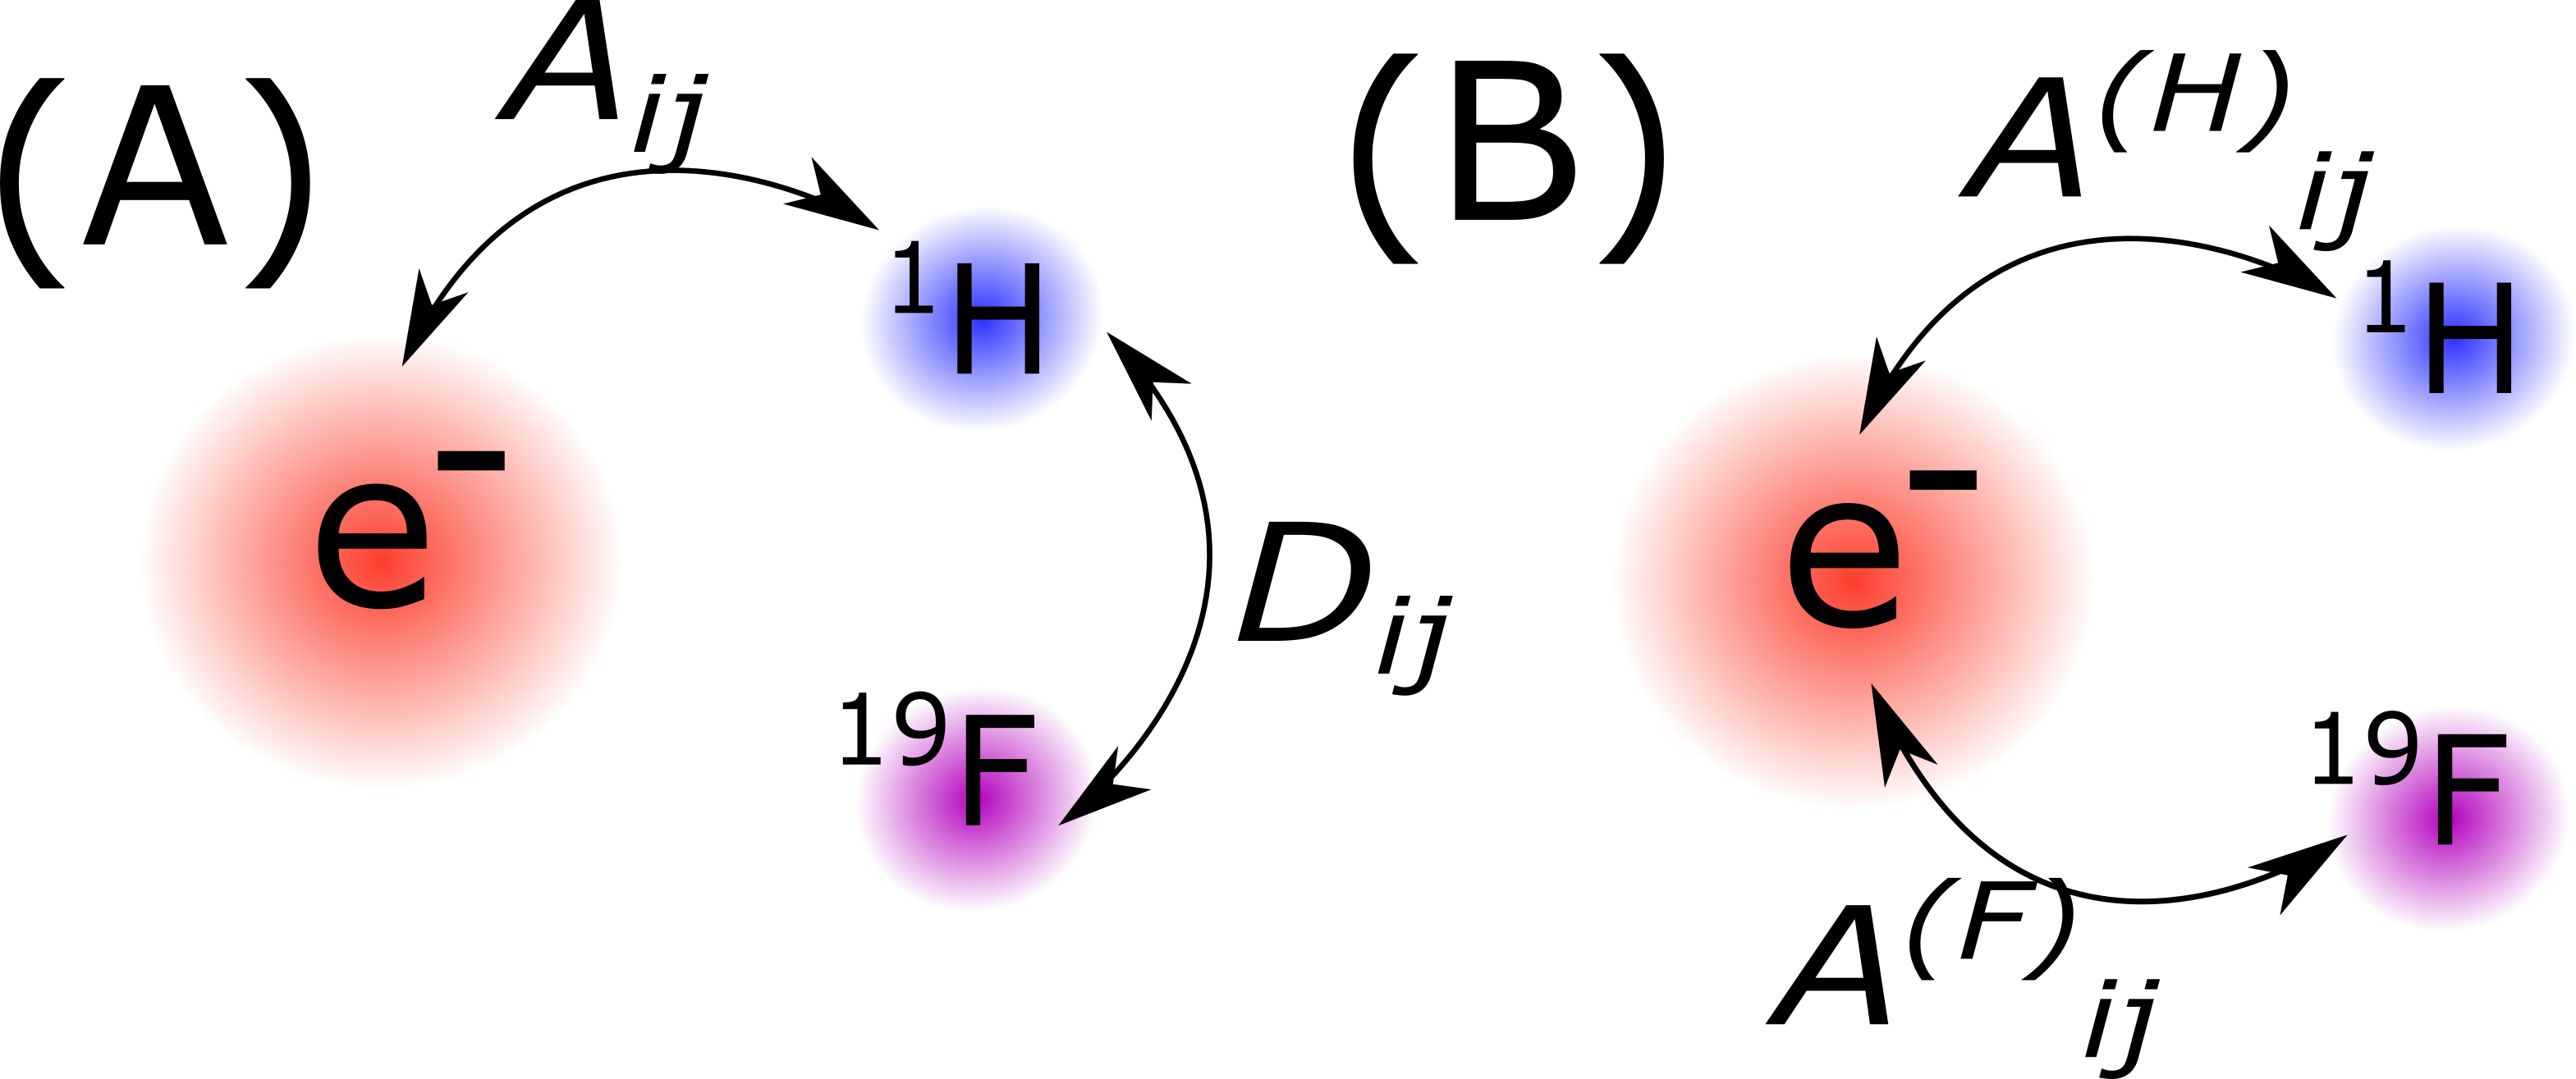
\includegraphics[scale=0.7]{text9330-7-6-8.png}
\end{figure}
%%%% END OF FIGURE

We neglect the hyperfine interactions of \textsuperscript{19}F nuclei at this stage to simplify the calculation, which corresponds to a case where \textsuperscript{19}F nuclei are sufficiently remote from the electron.The spin Hamiltonian for such a coupled three spin system can be written as: 
\begin{equation}
\mathcal{H} =  \omega_S \hat{S}_z + \sum_{i,j=x,y,z} A_{i,j} \hat{S}_i \hat{H}_j - \omega_H \hat{H}_z - \omega_F \hat{F}_z + \sum_{i,j=x,y,z} D_{ij} \hat{H}_i \hat{F}_j,
\end{equation}
where $\hat{H}_i, \hat{F}_i, \hat{S}_i$ - are the angular momenta of proton, fluorine and electron spins respectively. Taking into account that Electron Zeeman interaction is greater than any other terms, the Hamiltonian in the electron spin rotating frame would take a form:
\begin{equation}
\mathcal{H}  = A \hat{S}_z \hat{H}_z + B \hat{S}_z \hat{H}_x + D_{i,j} \hat{H}_i \hat{F}_j -  \omega_H \hat{H}_z - \omega \hat{F}_z + \sum D_{i,j=x,y,z} \hat{H}_i \hat{F}_j,
\end{equation}
where $A$ and $B$ are the secular and non-secular terms of the hyperfine interaction (term proportional to $\hat{S}_z \hat{H}_y$ was eliminated by a rotation in the spin space). The time-dependence in this Hamiltonian arises due to random flips of an electron spin, having a projection $m_S(t)=\pm \frac{1}{2}$ projection along the z-axis:
\begin{equation}
\mathcal{H} = (\omega_H + A m_S(t)) H_z + B H_x m_S(t) - \omega \hat{F}_z + \sum D_{i,j} \hat{H}_i \hat{F}_j
\end{equation}
The first two terms would collectively correspond to a quantization of a nuclear spin along a new effective magnetic field $\tilde{\mathbf{omega}}=(\omega_H + A m_S(t)),  B, 0)$. By rotating the spin operator around $\hat{H}_y$ by a small angle $\phi(t)= arctan(\dfrac{m_S(t)B}{\omega_H + m_S(t) A} )  \approx \dfrac{m_S B}{\omega_H}$ one can rewrite this part of Hamiltonian along the new axis: $B_z(t) \hat{H}_z + B_x(t) \hat{H}_x = \tilde{\omega}_H(t) \hat{\tilde{H_z}}$. The $\hat{H}_y$ operator generates a rotation in the spin space, the dipolar part of the Hamiltonian can will then be transformed as:
\begin{equation}
\begin{array}{lcl}
\hat{\tilde{H}}_{dip} (t) &=&  \exp(-i \phi(t) \hat{H}_y) \sum\limits_{i,j=x,y,z} D_{i,j} \hat{H}_i \hat{F}_j \exp(i \phi(t) \hat{H}_y)  \approx  \\
&\approx& \sum \limits_{i,j=x,y,z} D_{ij} \hat{H}_i \hat{F}_j+ \phi(t)[ \sum \limits_{i,j=x,y,z} D_{ij} \hat{H}_i \hat{F}_j, \hat{H}_y] \approx \\
&\approx& \sum \limits_{i,j=x,y,z} D_{ij} \hat{H}_i \hat{F}_j + \dfrac{m_S(t) B}{\omega_H} [ \sum \limits_{i,j=x,y,z} D_{ij} \hat{H}_i \hat{F}_j, \hat{H}_y]
\end{array}
\end{equation}
This time dependent Hamiltonian contains terms such as $\hat{H}_{\pm} \hat{F}_{\mp}$ and $\hat{H}_{\pm} \hat{F}_{\pm}$ is capable of inducing zero quantum (flip-flop) or double-quantum (flop-flop) transitions respectively. We will skip obtaining the exact equation for the rate, but rather focus in evaluating it by the order of magnitude. Using equation \ref{eq:rate} we can estimate the zero-quantum transfer rate as:
\begin{equation}
\begin{array}{cc}
W_{ZQ}  \sim \Big(  \dfrac{B D}{\omega_H} \Big) ^2 J(\omega_{ZQ}) \\
J(\omega) = \dfrac{\tau_c}{1+\omega^2\tau_c^2}
\end{array}
\end{equation}
where $B$ - is non-secular proton hyperfine interaction, $D$ - dipolar coupling, $ZQ$ stands for zero-quantum ($\omega_{ZQ} = \omega_H - \omega_F$), $\tau_c$.  We can now compare this rate to the electron-induced relaxation rate of nuclei $W_n = \dfrac{1}{T_{1n}}$ obtained in Eq.\ref{eq:nuclear__relax}:
\begin{equation}
W_{n}  \sim \vert B \vert ^2 J(\omega_F) \\
\end{equation}
Since $\omega_F \tau_c \gg 1$ and $\omega_{ZQ} \tau_c \gg 1$ ,  the spectral densities are equal to $J(\omega_F) \approx \dfrac{1}{\omega_F^2 \tau_c}$ and $J(\omega_{ZQ}) \approx \dfrac{1}{\omega_{ZQ}^2 \tau_c}$ . We can then look that the ratio of two rates, assuming that $\omega_H \approx \omega_F$:
\begin{equation}
\dfrac{W_{ZQ}}{W_n} \sim \Big( \dfrac{D}{\omega_H} \Big) ^2 \Big( \dfrac{\omega_F}{\omega_{ZQ}} \Big) ^2 \sim \Big( \dfrac{D}{\omega_{ZQ}} \Big) ^2
\end{equation}
Since a typical dipolar coupling is $D \sim 100 \text{ kHz}$ and $\omega_{ZQ} \sim 8 \text{ MHz}$, then $W_{ZQ} \ll W_n$ i.e. the $ZQ$ process is several orders of magnitude slower than nuclear relaxation rate $\dfrac{1}{T_1}$ thus a flip-flop in unlikely to occur during nuclear magnetization lifetime.  Similar argument is true for a double-quantum process. 


\section{Cross-relaxation due to level-crossings.}

As appears from Eq.\ref{eq:level_energies} the energy levels $E_2$ and $E_3$ could be rather close in energy, and could momentarily cross during the electron flip. We can neglect the perturbation $\hat{V}$ because it does not produce a significant mixing of levels ($\vert 2 \rangle$  and $\vert 3 \rangle$  in particular). 
The effective Hamiltonian for a system of two nuclei is:
\begin{equation}
	\mathcal{H}  = A_H m_S \hat{H}_z + B_H m_S \hat{H}_x -  \omega_H \hat{H}_z + A_F m_S \hat{F}_z + B_F m_S \hat{F}_x - \omega_F \hat{F}_z + D  ( \hat{H}_{z} \hat{F}_{z}  + \dfrac{1}{2}(\hat{H}_{+} \hat{F}_{-}  + \hat{H}_{-} \hat{F}_{+})),
\end{equation}
where $D$ is  a dipolar coupling. 
The Hamiltonian matrix in basis $\vert 1 \rangle, \vert 2 \rangle, \vert 3 \rangle, \vert 4 \rangle$ is:
{\tiny
\begin{equation}
    \hat{H}_{ik} = \begin{bmatrix}
    -\dfrac{\omega_H+\omega_F}{2} + \dfrac{m_S}{2}(A_H + A_F) + \dfrac{D}{4} & 0 & 0 & 0 \\
    0 & -\dfrac{\omega_H - \omega_F}{2} + \dfrac{m_S}{2}(A_H - A_F) - \dfrac{D}{4}& D & 0 \\
    0 & D & \dfrac{\omega_H - \omega_F}{2} - \dfrac{m_S}{2}(A_H - A_F) - \dfrac{D}{4} & 0 \\
    0 & 0 & 0 & \dfrac{\omega_H+\omega_F}{2} - \dfrac{m_S}{2}(A_H + A_F) + \dfrac{D}{4}    
    \end{bmatrix}
\end{equation}
}%
Let's focus on the evolution among states $\vert 2 \rangle$ and $\vert 3 \rangle$, where we could introduce some effective spin $\hat{I}^{(23)}$. The effective Hamiltonian driving the evolution of such a spin is:
\begin{equation}
   \hat{H}_{eff} = (-\dfrac{\omega_H- \omega_F}{2}  + \dfrac{m_S}{2}(A_H-A_F))\hat{I}_{z}^{(23)} + D   \hat{I}_{x}^{(23)},
\end{equation}
where diagonal dipolar interaction can be neglected because it is proportional to  an identity matrix.
This Hamiltonian  can be replaced with a classical vector model.  In this model, the rotation of magnetization in this model takes place around effective fields $\bm{\omega_{+}} = (D, 0, \Omega + a )$ and $\bm{\omega_{-}} = (D, 0, \Omega - a )$ depending on the electron state $m_S$, where $\Omega = \dfrac{\omega_H-\omega_F}{2}$ and $a = \dfrac{A_H-A_F}{4}$
Consider initial magnetization $\bm{M_0} = (0, 0, 1)$ at $t = 0$ aligned along z-axis, it rotates around $\bm{\omega_{+}}$ field, followed by a an electron flip at time $\tau_1$, rotation around $\bm{\omega_{-}}$ field for interval $\tau_2$ and a second electron flip. The rotation along the direction of $\omega_{-}$ would produce a vector:
\begin{equation}
\begin{array}{lcl}
      \bm{M}(\tau_1)  &=&  \bm{M_{\parallel}}  + \bm{M_{\bot x} }  \sin \omega_{+} \tau_1 + \bm{M_{\bot y}} \cos \omega_{+} \tau_1\\
      \bm{M_{\parallel}} &=& \dfrac{(\bm{M_0} \cdot \bm{\omega_{+}})}{  \mid \omega_{+} \mid ^2}  \bm{\omega_{+}} \\
      \bm{M_{\bot x}} &=&  \dfrac{(\bm{M_0} \times \bm{\omega_{+}})}{  \mid \omega_{+} \mid } \\
      \bm{M_{\bot y}} &=&        \bm{M_{0}} - \bm{M_{\bot x}} - \bm{M_{\parallel}},
\end{array}
\end{equation}
where $\bm{M_{\parallel}}$ is the  projection of vector $\bm{M_{0}}$  along the direction of $\bm{\omega_{+}}$, $\bm{M_{\bot x}}, \bm{M_{\bot y}}$ are directional vectors in the plane perpendicular to $\bm{\omega_{+}}$. Magnetization $\bm{M}$ will have a defined projection along the $\bm{\omega_{+}}$ and some additional component which orientation depends on $\tau_1$. 
An electron flip which follows next changes the direction of the effective field to $\bm{\omega_{-}}$, and magnetization continues to precess around this new direction. The component along the $\bm{\omega_{-}}$ can be found as:
\begin{equation}
    q = \dfrac{(\bm{\omega_{+}} \cdot \bm{\omega_{-}}  )}{ \mid  \bm{\omega_{+}}  \mid \cdot \mid \bm{\omega_{-}}  \mid    } =  \dfrac{D^2 + \Omega^2 - a^2}{\sqrt{D^2 + (\Omega + a )^2}  \sqrt{D^2 + (\Omega - a )^2}},
\end{equation}
while the rest of vector $\bm{M}$ will have a dependence on $\tau_1, \tau_2$. Since electron flips are random, then realization of a random process in different in various three spin systems, i.e. time intervals $\tau_1, \tau_2$ are random. Since $\tau_1, \tau_2 \sim \tau_c$ and $D \tau_c \gg 1$ the time-dependent component has a random orientation in various three spin systems, and averaging over ensemble produces zero (In other words, the zero-quantum nuclear coherences decay very rapidly).

Lets consider several scenarios.

\textbf{Scenario 1}.
If $D \ll \Omega, a, \mid \Omega - a \mid  $ the equation for $q$ simplifies to:
\begin{equation}
  q \approx 1 - \dfrac{D^2 a^2}{(\Omega^2 - a^2)^2}
\end{equation}
 After $n$ steps of random electron jumps taking place during interval $t =  n \tau_c $, the magnetization will decrease by a factor:
 \begin{equation}
    q^n = (1 - \dfrac{D^2 a^2}{(\Omega^2 - a^2)^2} )^n  = \exp \Big(-\ln (1 - \dfrac{D^2 a^2}{(\Omega^2 - a^2)^2}) n \Big) \approx \exp \Big[-\dfrac{D^2 a^2}{(\Omega^2 - a^2)^2} \dfrac{t}{ \tau_c} \Big]
 \end{equation}
 In other words the rate of nuclear flip-flop is $W_{ff} = \dfrac{D^2 a^2}{(\Omega^2 - a^2)^2} \dfrac{1}{ \tau_c} $. Taking the ratio of a flip-flop rate and nuclear relaxation rate and taking into account that non-secular and secular hyperfine are of the same order of magnitude  $B  \sim a$ one obtains:
 \begin{equation}
    \dfrac{W_{ff}}{W_n} \approx ( \dfrac{D \omega_H}{\Omega^2 - a^2} )^2
 \end{equation}
 For the smallest $a \ll \Omega$ under our experimental conditions is $ \dfrac{W_{ff}}{W_n} \ll 1$. For nuclei located closer to the electron and thus having larger hyperfine couplings $ \dfrac{W_{ff}}{W_n} \approx 1$. 
 
\textbf{Scenario 2}.

However, there is chance that some nuclear pairs have frequency difference  $a \approx \Omega$. For those the value of $q = \dfrac{D}{\sqrt{D^2 + 4 \Omega ^2}} \ll 1$. In practice it means that for one of the electron $m_S$ states the levels of nuclear subsystem become degenerate and large $D$ mixes them very rapidly.

\textbf{Scenario 3}.
In principle the treatment equally applies to level crossings for nuclei of one type, such that $\omega_H = \omega_F$, $\Omega = 0$. In this case $q$  becomes:
\begin{equation}
  q = \dfrac{D^2 - a^2 }{D^2 + a^2}
\end{equation}
For small $D \ll a$ this can be simplified as $q \approx 1 - \dfrac{D^2}{a^2}$, and the ratio of a flip-flop rate to nuclear relaxation time is:
\begin{equation}
    \dfrac{W_{ff}}{W_n} \approx ( \dfrac{D \omega_H}{a^2} )^2
\end{equation}
For $a \approx 3$ this ratio becomes $\approx 1$ and for smaller $a$ it becomes even bigger. In practice it means that \textbf{flip-flops among nuclei of one kind are very likely to occur within nuclear magnetization lifetime}.





\section{Conclusions.}

We have explored three potential mechanisms for cross-relaxation and have discovered that the most potent mechanism of cross-relaxation is produced by rapid level crossings of \textsuperscript{19}F and \textsuperscript{1}H nuclei, brought about by random electron jumps. 

  

\end{document}
